\chapter{背侧前额叶皮层:基于最近事件生成目标}
背侧PF皮层有助于根据顺序、时间和空间环境生成目标,它的连接解释了为什么只有它才能做到这一点。背侧PF皮层,包括中外侧PF皮层(46区),通过与后顶叶皮层、前运动皮层和PF皮层的其他部分连接来发挥作用。顶叶连接提供了许多用于生成目标的空间和时间背景。与运动前区域的联系导致这些目标的实现,通常是通过手的运动。与眶侧PF皮层的连接使背侧PF皮层能够根据单个事件预测目标选择的具体结果。背侧PF皮层位于背侧视觉流的末端,因此它可以规划目标序列,它可以具体或抽象地指定这些目标。在产生目标后,背侧PF皮层可以前瞻性地编码它们,直到行动的时候到来。鉴于背侧PF皮层在类人猿灵长类动物中进化(第2章),我们认为它在使用最近视觉事件的顺序、时间和位置来指导觅食选择和生成效率优化的目标序列方面具有优势。

\section{介绍}
第二章解释了灵长类动物的PF皮层在类人猿中随着新区域的出现而扩展。第三章涉及了其中的一些,例如极性PF皮层(10区),但在本章和下一章,它们是主要主题。由于类人猿依赖于白天漫长的觅食旅行,它们需要消耗大量的能量,并面临着很高的捕食风险。这种生活方式非常重视正确的觅食选择。在影响这种选择的因素中,视觉事件的位置、时间和顺序是突出的,因为类人猿利用了它们在中央凹和色彩视觉方面的进步。正如第二章所解释的,这些进步包括中央凹提供的精致的视觉敏锐度和三色视觉提供的增强的辨别能力。

这一章解释了觅食的选择部分取决于当前的环境,这是由选择时可用的刺激以及最近视觉事件的记忆所指定的。为了理解我们的意思,考虑一个简单的实验室任务:延迟匹配样本。猴子把一个刺激看作一个样本,然后看到一个或多个刺激需要选择。这种选择不仅取决于选择时的刺激,还取决于基于样本刺激的记忆。这两个因素共同构成了当前选择目标的背景。

由于记忆对当前情境起作用,这类实验的被试面临一个问题:最近发生了几件事,并选择了几个目标。本章的大部分内容探讨了背侧PF皮层如何帮助类人猿灵长类动物解决这个问题。许多文献都依赖于一个任务和一个区域:延迟反应任务,它依赖于中外侧PF皮层(46区)。因此,我们将讨论的重点放在第一章和第五章也提到的这个任务上。我们认为,因为受试者在这个任务中经历了一系列的视觉事件,并实现了一系列的目标,他们需要挑选出决定当前目标的事件。然后,我们回顾一系列其他任务,这些任务也要求主体在当前环境的基础上生成目标。
\section{区域}
在猕猴中,中外侧PF皮层位于主枕沟的吻侧三分之二(图6.1)。然而,它也延伸到这个沟的背侧和腹侧的凸面皮层。中外侧PF皮层(46区)有很多名字,有些很明确,有些则不太明确。
\begin{figure}
	\centering
	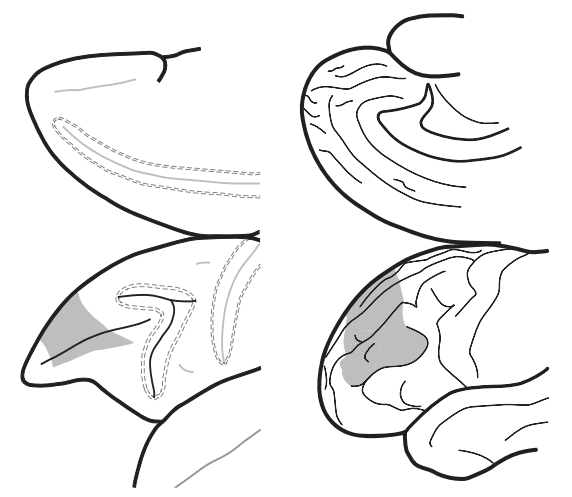
\includegraphics[width=0.7\linewidth]{image_pfc/Fig_6_1}
	\caption{猕猴(左)和人类(右)的背侧PF皮层。格式如图1.2所示。}
	\label{fig:fig}
\end{figure}

Walker(1940)将沿主沟整个长度的皮层称为46区,但最近Petrides和Pandya(1999)将9/46区区分为该沟的尾端周围(见图1.2)。为了避免对46这个术语的不同用法的混淆,我们称沃克46区吻侧三分之二为中外侧PF皮层,尾侧三分之一为后外侧PF皮层。在人类中,这些分区位于额上回和额下沟之间。

尽管出现了这些新术语,但混淆的空间仍然很大。术语背侧前额叶皮层最初是指猴子的整个侧前额叶皮层(Pribram et al. 1952),但后来仅指主沟内和背侧的皮层(Mishkin et al. 1969)。在影像学文献中,指PF背外侧皮层已变得很常见,但该术语的使用通常非常松散,很少注意解剖标志。因此,我们在本书中避免使用这个术语。表1.2给出了我们所采用的术语。我们将PF背侧皮层包括主沟两岸的皮层和其背侧的凸面皮层(区域9),但不包括区域9的内侧部分。当然,这些划分并不是最终的结果,但它们在一定程度上反映了联系。
\section{连接}
图6.2展示了PF皮层背侧的一些皮质连接。正如第一章所解释的,这些连接构成了解剖指纹。
\par
1.中外侧PF皮层(46区)与后顶叶皮层,特别是尾顶叶区有很强的联系(Petrides \& Pandya 1984,1999,2009)。正如前一章所提到的,后顶叶皮层的许多神经元编码视觉空间信息。然而,顶叶细胞也编码时间间隔(Leon \& Shadlen 2003),当人类受试者对近期事件做出判断时,左侧顶叶内沟会出现激活(Dudukovic \& Wagner 2007)。
\par
2.中外侧PF皮层连同外侧9区,与位于颞上沟上岸的多模态区TPO区(也称为颞上多感觉区STP)相连(Seltzer et al. 1996;Petrides \& Pandya1999)。该区域的细胞对体感、听觉和视觉刺激有反应(Bruce et al. 1981)。
\par
3.中外侧PF皮层也接受来自周围皮层的输入(Petrides \& Pandya 1999),其功能是识别物体(Murray et al. 2007)。这种联系表明,中外侧前额叶皮层接收到有关物体的直接输入,而不仅仅是腹侧前额叶皮层的间接输入(第7章和第8章)。
\par
4.中外侧前额叶皮层接收来自次级体感觉区(S2) (Petrides \& Pandya 2002b)和下颞叶皮层吻侧PFG区(Rozzi etal . 2006)的输入。这些区域的细胞对体感刺激有反应(Hyvarinen 1981),中外侧PF皮层的细胞也是如此(Tanila et al. 1993)。这一特征将中外侧PF皮层与尾侧和后外侧PF皮层区分开来,后者的细胞主要具有视觉和注意力特性(第5章)。
\par
5.中外侧PF皮层连接背侧和腹侧前运动皮层(Wang et al. 2002),以及前辅助运动区(preSMA) (Wang et al. 2005)和位于扣带沟的扣带吻侧运动区(CMAr) (Dum \& Strick 1993)。这些投影主要涉及代表手和手臂的运动前区域,而不是脚和腿。前肢表征的专门化表现在背侧前前皮层的吻侧部分(Tachibana et al. 2004)、腹侧前运动皮层(He et al. 1993)、preSMA (Luppino et al. 1991)和CMAr (He et al. 1995)。因此,相对于运动的运动,中外侧PF皮层在伸手、操作和进食运动中具有优先的作用(第2章)。
\par
6.中外侧PF皮层与前扣带皮层有很强的联系(Petrides \& Pandya 1999)。第3章解释了前扣带皮层在动作的评估和基于这些评估的动作之间的切换中发挥作用(Walton et al. 2007)。
\par
7.中外侧PF皮层与脾后皮层相连(Morris et al. 1999)。反过来,从脾后皮层投射到海马旁回和下丘前(Kobayashi \& Amaral 2007)。我们认为,这些联系可能在有关事件的记忆检索中发挥作用,而这种检索依赖于时间或空间上下文(Vann et al. 2009)。
\par
8.区域9的横向部分的连接受到的关注相对较少,部分原因是很少有功能数据引起人们的兴趣。这部分背侧PF皮层与背侧运动前皮层的吻侧部分(Petrides \& Pandya 1999)和CMAr (Morecraft \& van Hoesen 1993)有联系。就像第9区域的内侧部分一样,它也与上颞皮质有联系,这可能传达听觉信息(Petrides \& Pandya 1984;Saleem et al. 2008)。最后,第9区外侧部分与后顶叶皮层下部(PG区)(Cavada \& Goldman-Rakic 1989)和脾后皮层(Kobayashi \& Amaral 2003)相连。
\begin{figure}
	\centering
	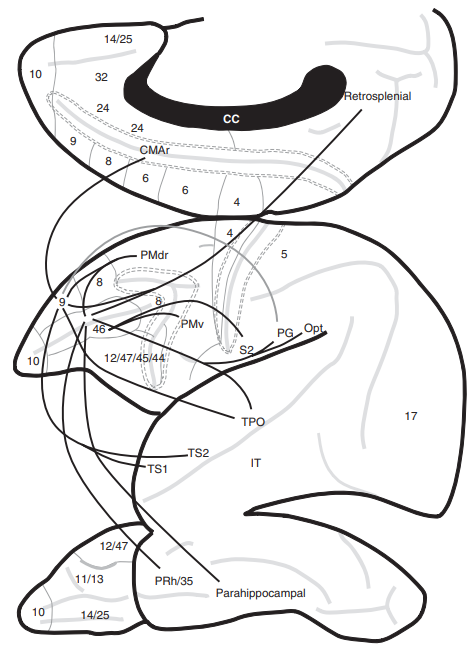
\includegraphics[width=0.5\linewidth]{image_pfc/Fig_6_2}
	\caption{PF皮层背侧的选定连接。图1.4和1.5给出了沟和区域的名称。一些轴突与背侧PF皮层有直接连接的区域被认为是相互的,除非另有说明。}
	\label{fig:fig}
\end{figure}

\subsection{总结}
中外侧PF皮层与后顶叶皮层、前运动皮层有很强的联系,并间接与海马系统有联系。它也与PF皮层的其他部分相互连接,如眶PF皮层。其他皮质区域没有这种连接模式。因此,它很好地整合了由眶前PF皮层、背侧视觉流和海马体处理的信息,并向运动前皮层提供信息。

\section{延迟响应任务}
中外侧前额叶皮层在接收后顶叶皮层的视觉空间信息方面与尾侧前额叶皮层相似。因此,任何一个区域的损伤都会导致猴子在动眼延迟反应任务和经典版本的延迟反应任务上的表现中断,这并不奇怪。在这两项任务中,空间线索指导目标选择,猴子必须在可能的空间目标中进行选择。当然,根据定义,动眼肌延迟反应任务需要对目标进行扫视,而经典的延迟反应任务需要达到目标的运动。第5章解释了尾侧PF皮层和后外侧PF皮层的损伤会导致动眼力延迟反应任务的准确性误差,根据它们与背侧视觉流的连接,这是有意义的。这些损伤不会引起很多明显的错误,当它们发生时,猴子会迅速纠正这些错误(Tsujimoto \& Postle 2012)。

相反,中外侧PF皮层(46区)的永久性损伤对经典的延迟反应任务造成毁灭性的损害。当猴子在手术前学习延迟反应任务时,它们在中外侧PF皮层损伤后执行任务的效果并不比偶然水平好(Goldman \& Galkin 1978)。也就是说,受损的猴子犯的错误和正确的选择一样多。当他们在中外侧PF皮层持续受损后第一次尝试学习任务时,即使有短暂的(1秒)延迟期,他们也无法完成任务(Battig et al. 1960)。而且它们永远无法恢复,至少在任何人测试过的时间范围内都无法恢复。

一个重要的方法差异可以解释这种差异的部分原因。在经典的延迟反应任务中,猴子伸手去拿盖在食物井上的盖子。这意味着在这个版本的任务中,不像动眼肌延迟反应任务,受试者只能犯明显的错误。精度错误,如果发生,将不会被记录。

另一个区别可能也很重要。猴子可以通过在延迟期间偷偷地关注目标位置来解决动眼肌延迟反应任务。但是实验者执行经典延迟反应任务的方式使得隐蔽注意力很难集中到目标上。传统的测试方法包括威斯康星通用测试装置(WGTA)。在该装置中,一个不透明的屏幕在延迟期间下降,使猴子在延迟期间无法看到相关位置(图6.3)。在神眼运动版本的任务中,猴子可以在周边视觉中看到目标位置,尽管在扫视时它不再被标记出来。

原则上,执行经典延迟反应任务的猴子仍然可以准确地注意到WGTA的目标一侧,或者以某种方式将姿势定向到那一侧。然而,降低屏幕往往会导致猴子在测试室内移动。Passingham(1971)在延迟期间监测了正常猴子的位置,发现即使它们已经解决了问题,在40\%的试验中,它们也会从房间的一边穿过到另一边。因此,猕猴不需要通过身体定位来解决延迟反应任务所带来的问题,似乎测试方法很可能排除了使用隐蔽注意力来解决这个问题。因此,动眼肌延迟反应相对缺乏坦率的错误可能反映了隐蔽地关注目标位置的持续能力,而延迟反应任务的经典版本的严重损害可能是由于破坏了这一策略。

当然,延迟响应任务可以在没有不透明屏幕的情况下呈现。在延迟期间,食物井可能在受试者够不到的地方。在这种情况下,猴子似乎更有可能采取某种姿势或注意力的方法来弥合延迟期,或者使用其他策略来做到这一点。Wilson et al.(1963)发现。正常的猴子在延迟期开始时坐在测试室的正确一侧,在延迟期结束时仍保持在该一侧。然后,当他们有机会这样做时,他们就会到达离目标最近的距离。在延迟开始时,有PF皮层损伤的猴子也坐在正确的一侧,但在延迟结束时,它们到达相反(错误的)目标的次数与到达正确目标的距离较短的次数一样多。这一发现表明,对于有PF损伤的猴子来说,姿势或注意力的延迟期桥接不足以正确地形成延迟反应任务。

目前还不清楚为什么猴子在整个延迟期间不采取保持在WGTA正确一侧的策略。这个策略可以解决问题。也许他们没有意识到,他们在延迟期开始时看到的东西表明了他们在延迟期结束时应该达到的目标。换句话说,受损的猴子可能无法识别延迟间隔之前的视觉事件与它们即将做出的选择有任何关联。正常的猴子确实认识到这种关系,并且不需要采取姿势定向策略或注意力策略来执行任务。

在后面的部分中,我们提出了这样的想法,即为了解决延迟响应任务所带来的问题,猴子需要知道延迟期之前的视觉事件为它们之后选择目标提供了关键。我们认为,中外侧前额叶皮层受损的猴子要么无法学习这一规则,要么无法记住和应用它。

\begin{figure}
	\centering
	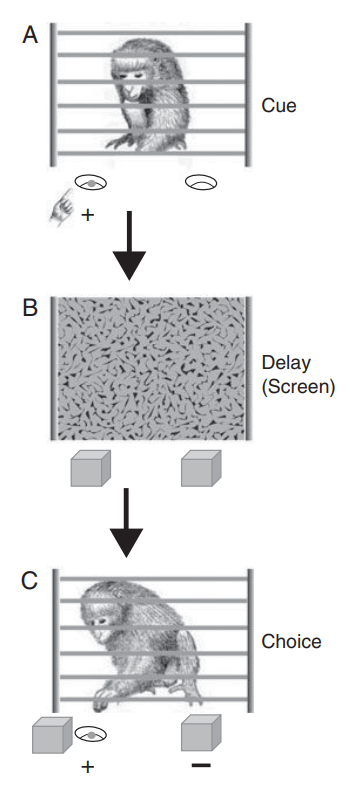
\includegraphics[width=0.2\linewidth]{image_pfc/Fig_6_3}
	\caption{在威斯康星州通用测试装置(WGTA)中延迟响应任务的测试程序。(A)实验员在两个食物井(+)中的一个上饵,一只猴子从它的测试笼中观察。这个动作作为视觉提示事件。(B)实验者在延迟期间放下一个不透明的屏幕。相同的物体可以很好地覆盖食物。(C)实验者举起屏幕后,猴子在两个食物井中进行选择,将其中一个物体移开,如果正确(+)则获得奖励,如果错误(-)则得不到奖励。修改自Murray EA.杏仁核复合体对猕猴行为的贡献。脑研究进展87:167-80©1991,Elsevier许可。}
	\label{fig:fig}
\end{figure}
\subsection{延迟期的重要性}
第5章提到,尽管尾侧PF皮层病变的猴子在动眼力延迟反应任务上只有轻微的损伤,但它们在没有延迟期的条状视动任务上也有损伤。相比之下,在中外侧前额叶皮层有损伤的猴子只在包括延迟期的任务中有损伤。

Passingham (1985a)设计了一个没有延迟的条件视觉运动任务。显示器中央的两个面板,一个在另一个上面,提供线索。猴子们知道,如果光出现在顶部的面板上,那么它应该选择一侧的目标;如果一个光出现在底部面板,那么它应该选择另一边的目标。所以这个任务包括空间线索和空间目标就像延迟反应任务一样,但不像延迟反应任务它不包括延迟期。中外侧和后外侧PF皮层病变的猴子可以正常学习这项任务。

Stamm(1969)的结果也表明,延迟是产生损伤的关键因素。在一个试验中,他在不同的时间点灭活了中外侧或后外侧前额叶皮层。在延迟期的早期,中外侧PF皮层(46区)的破坏估计导致延迟反应任务的表现下降到机会水平。刺激后外侧皮层效果较小。这一发现与巴特斯(Butters)和潘迪亚(pandya)(1969)的一项研究结果一致,他们在该研究中表明,主沟中央三分之一的病变导致延迟交替任务的严重损害,而后三分之一的病变的影响要小得多。

综合来看,这些结果支持两个结论。首先,延迟响应任务的损害确实是由于延迟期的强加造成的。其次,中外侧PF皮层在这一任务中起着必要的作用。在密切相关的延迟交替任务中也是如此。
\subsection{延迟周期活动}
关于延迟反应障碍,最常被引用的说法是猴子无法记住线索的位置,因此这种缺陷可以被描述为回溯性空间工作记忆的缺陷之一。人们可以记录下延迟期间的活动,而且乍一看,这种活动似乎是对线索位置的记忆编码,这一事实被解释为支持这一结论的证据。然而,这种活动发生在PF皮层的许多部分,以及其他区域。第五章解释了延迟期活动并不总是编码空间记忆。当研究人员在充分的比较条件下研究细胞活动时,他们可以看到大部分所谓的记忆活动实际上编码了参与的位置。然而,一些延迟期活动确实编码了记忆的位置,因此,中外侧PF皮层的延迟期活动仍然有可能介导回溯性工作记忆。

Kojima和Goldman-Rakic(1984)从中外侧PF皮层(46区)进行记录,试图验证空间工作记忆理论。他们使用了两种条件。在一种情况下,线索在延迟期间消失,而在另一种情况下,线索在整个试验过程中仍然可见。在延迟期间编码位置的62个细胞中,当刺激仍然可见时,44个细胞表现出相同或更大的延迟期活动。当刺激消失时,只有12个细胞更活跃。Tsujimoto和Sawaguchi (2004b)在类似条件下使用了动眼肌延迟反应任务,并证实了这一结果模式。

对这一发现最有可能的解释有四种:
\par
1.即使线索仍然可见,也没有什么能阻止猴子“记住”它的位置。因此,在这两种情况下,它们可能会“记住”提示的位置。
\par
2.在这两种情况下,猴子可能会盯住目标。Kojima和Goldman-Rakic(1984)没有记录眼睛的位置,所以我们不能排除他们的结果是由于明显的注意力。
\par
3.在这两种情况下,猴子可能会偷偷地关注目标。
\par
4. 在这两种情况下,猴子可能会对空间目标的位置进行编码。这种表述可能包括一个计划好的行动,也可能独立于实现目标所需的行动而指定目标。

在这四种解释中,只有第一种与Kojima和Goldman-Rakic(1984)的解释是一致的。他们得出的结论是,延迟期的活动反映了线索在回顾记忆中的位置,这与空间工作记忆理论一致。然而,猴子似乎不太可能“记住”它们能看到的刺激。第二种说法,就公开关注而言,可以解释小岛和戈曼-拉基奇的结果,但不能解释辻本和泽口的结果。在后一项研究中,猴子必须在整个延迟期间固定在一个中心位置。第三种解释,即隐性注意,也可以解释两项研究的结果,但它与回溯性工作记忆方面的解释不相容。

这就剩下了第四种解释,它将延迟期活动解释为反映了空间目标的位置,这是Fuster(1973)首次提出的。换句话说,这表明延迟期反映的是前瞻性记忆,而不是回顾性记忆。猴子每天进行多次试验,这意味着先前试验的线索和目标位置在记忆中相互干扰。在任何特定的试验中,只要看到线索,猴子就能通过编码目标位置来克服这种干扰。

第五章回顾了一些似乎反对目标的前瞻性编码的证据。大多数细胞编码反眼跳任务中的线索位置,只有少数编码目标位置。在另一项研究中,细胞对提示位置进行编码,即使这些位置不是未来的目标。然而,这些研究都没有明确地关注中外侧PF皮层的细胞,而不是后外侧或尾侧PF皮层。

在本章稍后将详细介绍的一项研究中,Genovesio等人(2006a)确实研究了中外侧PF皮层中的细胞,以及其他神经元种群,他们的实验设计允许他们区分位置的回顾性编码和前瞻性编码。他们发现,中外侧前额叶皮层的细胞尽可能快地编码当前的目标位置,并且回溯编码在这个时候消失。我们还在后面的一节中提供数据,表明这种预期的活跃度可以防止内存干扰(Sakai et al. 2002a)。

\subsection{总结}
中外侧PF皮层损伤的猴子在机会水平上执行延迟反应任务,并且它们没有恢复。在延迟期间的破坏性电刺激会导致损伤,在没有延迟期的任务中,猴子表现正常。延迟期活动发生在中外侧PF皮层,它编码一个位置。这种活动已经被解释为回顾性空间记忆,但证据表明,这种活动也编码了当前目标的位置(预期编码)和参与的位置。

\subsection{活动和激活}




\subsection{结论}


